\subsection{How to make a type checker incremental?}

\begin{frame}
  \begin{center}
    \large
    {\bf Problem 1:}
    How to make a type checker incremental?
  \end{center}
\end{frame}

\begin{frame}{\textcolor{gray}{Certificates for incremental} type-checking}

  \begin{block}{Observations}
    \begin{itemize}
    \item Program elaboration is more and more an \emph{interaction}
      between the programmer and the type-checker
    \item The richer the type system is, the more expensive
      type-checking gets
    \end{itemize}
    \begin{example}
      \begin{itemize}
      \item type inference (\eg\ \sysname{Haskell}, unification)
      \item dependent types (conversion, esp. reflection)
      \item very large term
      \end{itemize}
    \end{example}
  \end{block}
  \pause
  \begin{center}
    \large \emph{\ldots but is called repeatedly with \emph{almost} the same input}
  \end{center}
\end{frame}

\begin{frame}{\textcolor{gray}{Certificates for incremental}
    type-checking}
  \vspace{0.5em}
  \begin{center}
    \only<1>{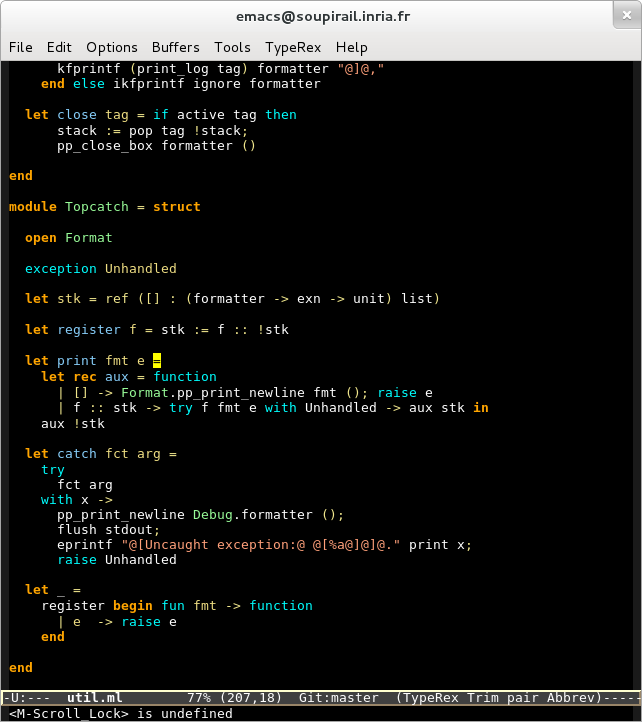
\includegraphics[height=0.9\textheight]{images/emacs1.png}}%
    \only<2>{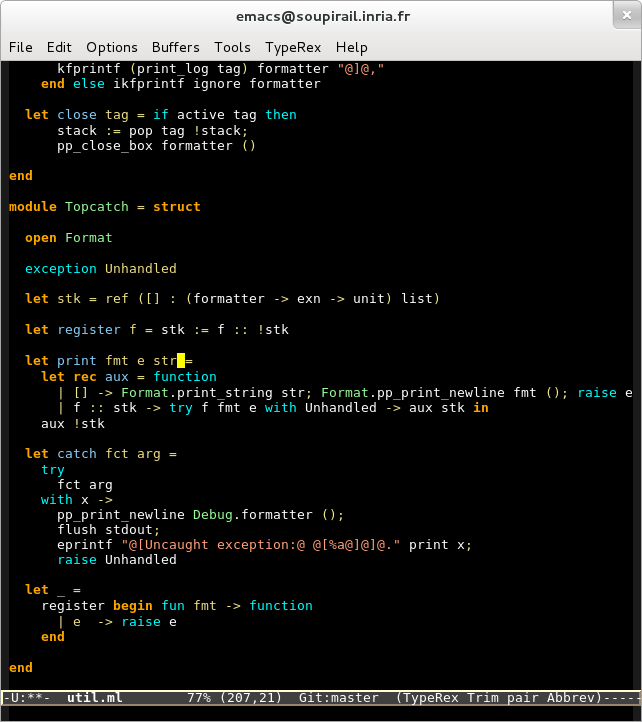
\includegraphics[height=0.9\textheight]{images/emacs2.png}}%
    \only<3>{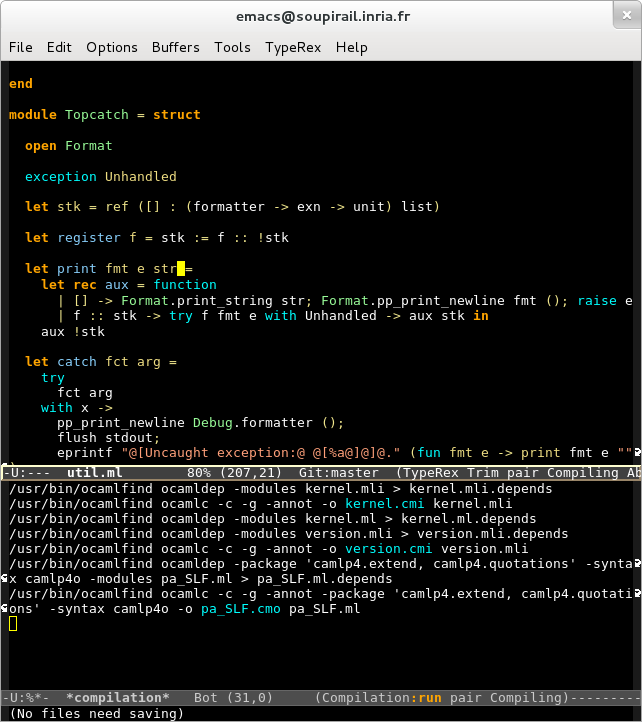
\includegraphics[height=0.9\textheight]{images/emacs3.png}}%
    \only<4>{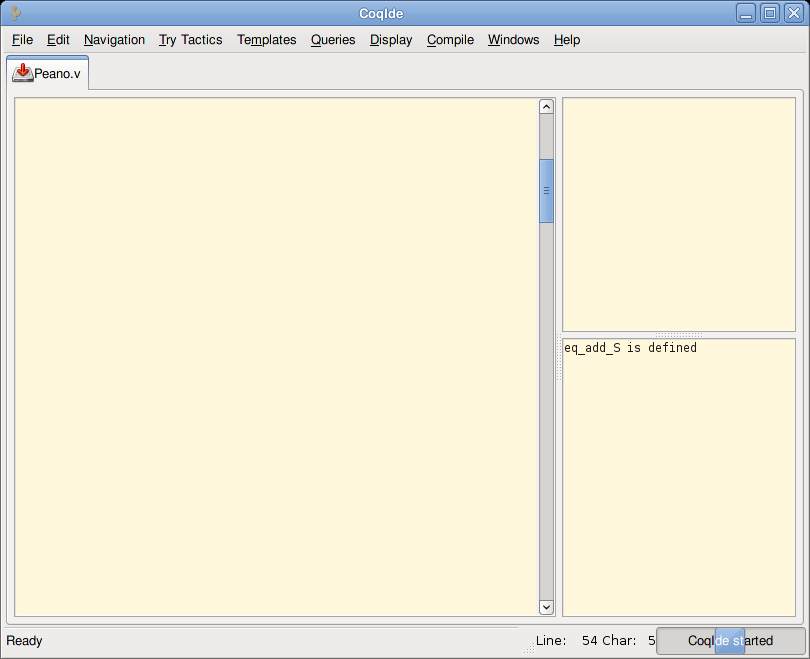
\includegraphics[width=0.85\textwidth]{images/coqide00.png}}%
    \only<5>{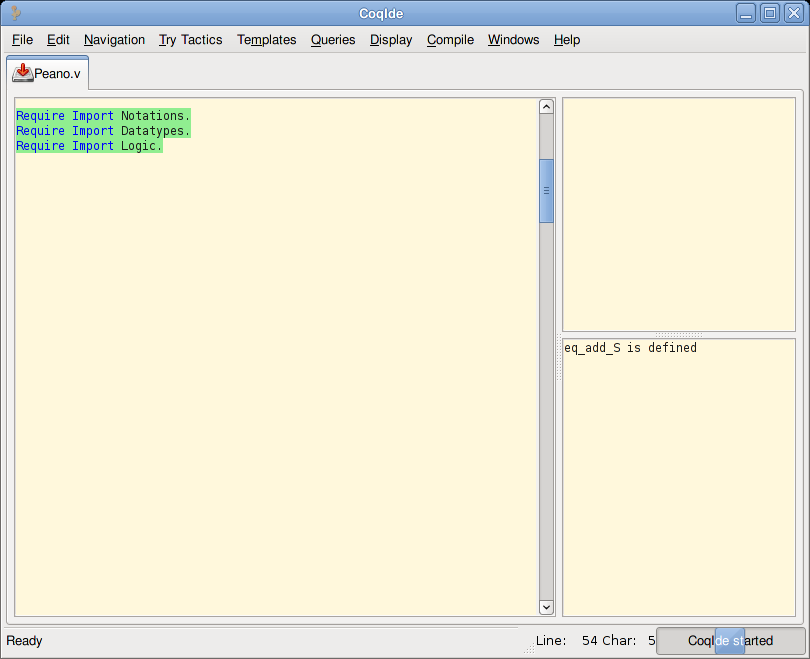
\includegraphics[width=0.85\textwidth]{images/coqide0.png}}%
    \only<6>{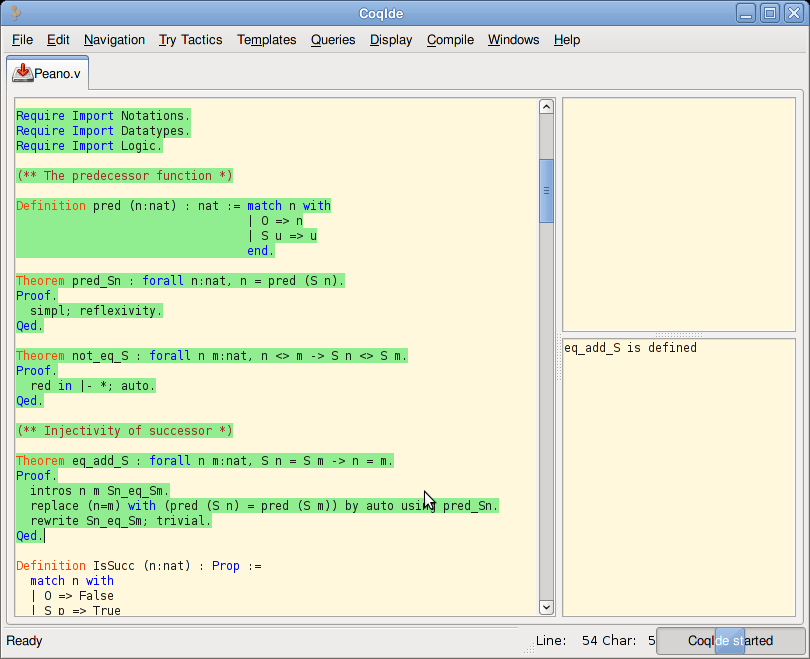
\includegraphics[width=0.85\textwidth]{images/coqide.png}}%
    \only<7>{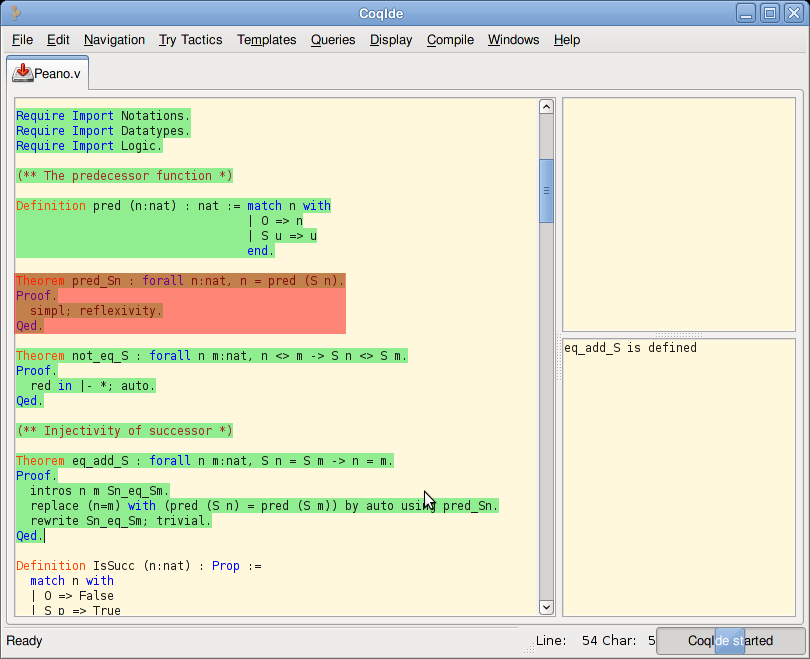
\includegraphics[width=0.85\textwidth]{images/coqide2.png}}%
    \only<8>{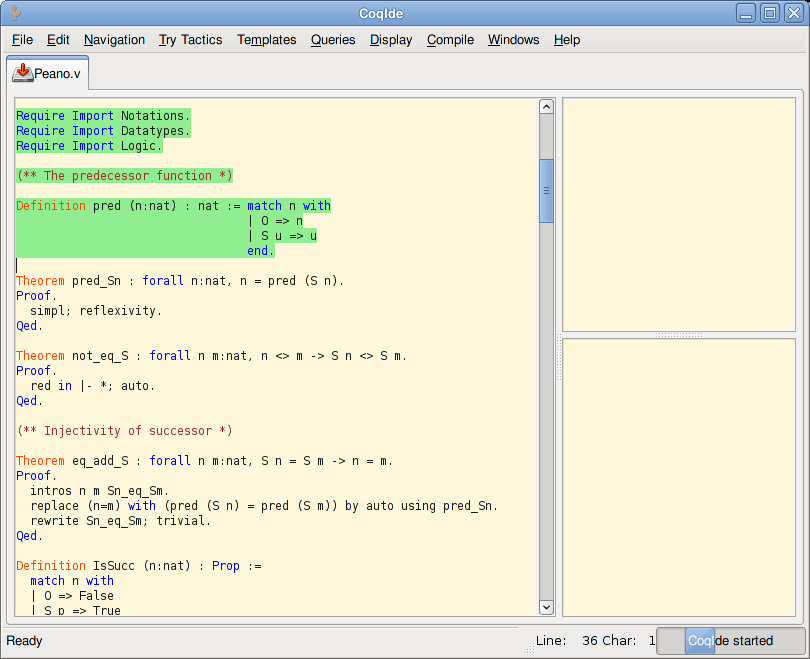
\includegraphics[width=0.85\textwidth]{images/coqide4.png}}%
    \only<9>{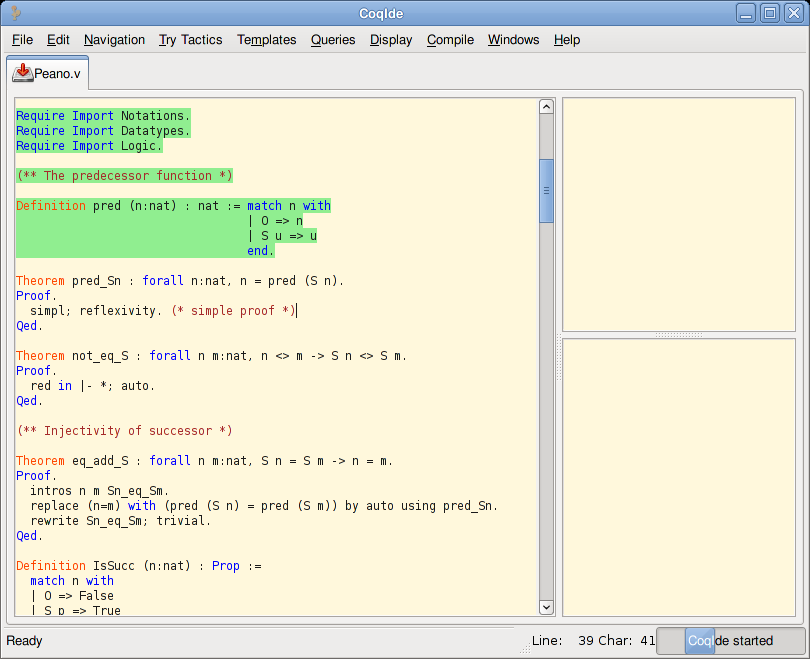
\includegraphics[width=0.85\textwidth]{images/coqide5.png}}%
    \only<10>{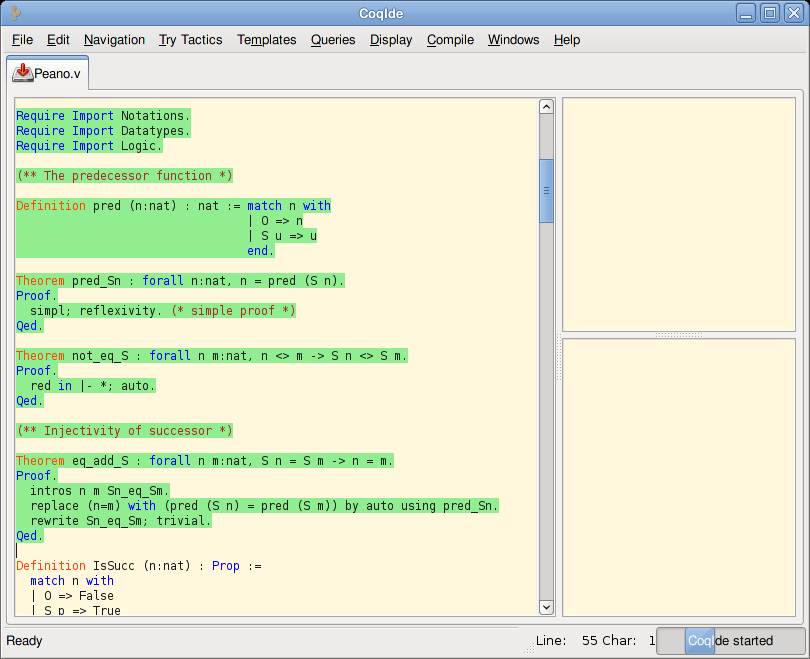
\includegraphics[width=0.85\textwidth]{images/coqide6.png}}%
    \only<11>{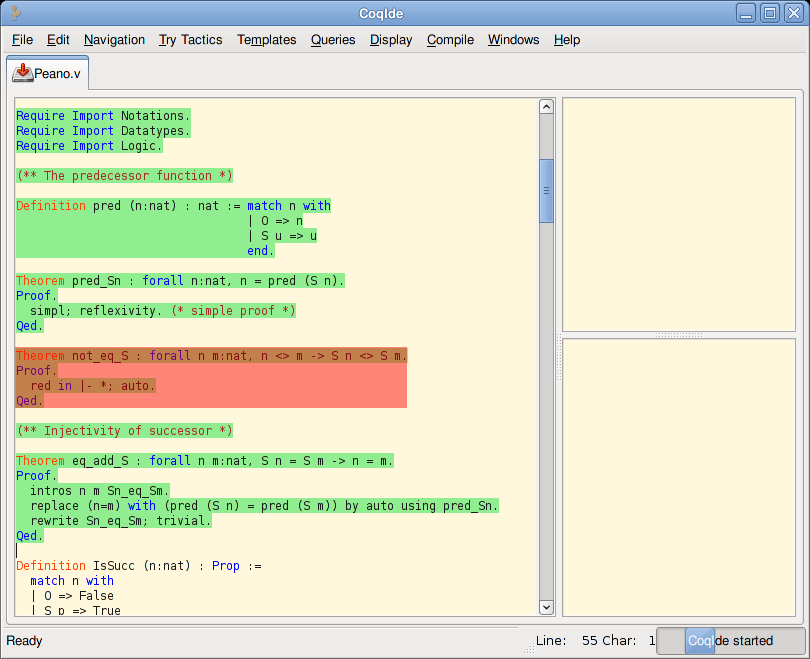
\includegraphics[width=0.85\textwidth]{images/coqide7.png}}%
  \end{center}
\end{frame}


\begin{frame}{\textcolor{gray}{Certificates for} incremental
    \textcolor{gray}{type checking}}

    \begin{block}{Problem}
      \emph{How to take advantage of the knowledge from previous type-checks?}
      \begin{itemize}
      \item Reuse already-computed results
      \item Recheck only the changed part of a program and its
        \emph{impact}
      \end{itemize}
    \end{block}
\end{frame}

\subsection{How to trust your type checker?}

\begin{frame}
  \begin{center}
    \large
    {\bf Problem 2:}
    How to trust your type checker?
  \end{center}
\end{frame}

\begin{frame}{A compiler designer's job}
  \begin{center}
    \begin{tikzpicture}[auto, >=latex]
      \node (ts) {System \sysname{Z}};

      \node (tc) [below=4em of ts] {$\tt \finfer\ :\ \cst{env} \to \cst{tm} \to \app
        {\cst{tp}} \cst{option}$};

      \path[->] (ts) edge (tc);
    \end{tikzpicture}

    \vspace{2em}
    set of declarative inference rules $\to$ decision algorithm
  \end{center}
  \pause
  \begin{itemize}
  \item non trivial (inference, conversion\ldots)
  \item critical
  \end{itemize}

\end{frame}

\begin{frame}{\textcolor{greenish}{Example:} System \sysname{T}$_{<:}$}
  \begin{block}{Syntax}
    \vspace{-2em}
    \begin{align*}
      M &\gequal \z \gor \s M \gor M M \gor \lam x M \gor
      \recb M N x y P \\
      A &\gequal \nat \gor \even \gor \odd \gor A \to A
    \end{align*}
  \end{block}
  \begin{block}{Typing rules}
    \vspace{-2em}
    \begin{mathpar}
      \infer{\jts M \nat \and \jts N A \and \infer*{}{\mbox{$
            \begin{array}{c}
              [\jts {\var x} \nat] \quad
              [\jts {\var y} A] \\[-0.3em]
              \vdots\\
              \jts P A
            \end{array}
            $}} }{\jts {\recb M N x y P} A}

      \only<2>\alert{\infer{\jts M A \and \jsub A B}{\jts M B}}

    \end{mathpar}
  \end{block}
  \pause
  \begin{center}
    {\large\it \alert{Not syntax directed!}}
  \end{center}
\end{frame}

\begin{frame}{\textcolor{greenish}{Example:} System \sysname{T}$_{<:}$}
  \begin{block}{Typing algorithm}
    \begin{overlayarea}\textwidth{8em}
      \large \only<1>{$$ \infer{\Gamma\jts M {A\to B} \and \Gamma\jts
          N A}{\Gamma\jts{\app M N} B}
    $$}

  \only<2>{$$ \infer{ \Gamma\jts M {A\to B} \and \infer*{ \Gamma\jts N
        {A'} \and \Gamma\jsub {A'} A }{ \Gamma\jts N A } }{
      \Gamma\jts{\app M N} B }
    $$}

  \only<3>{$$ \infer{ \Gamma\jts M \nat \and \Gamma\jts N A \and
      \Gamma, \var x :\nat, \var y: A\jts P A }{\jts {\recb M N x y P}
      A}
    $$}

  \only<4->{$$ \infer{ \Gamma\jts M {T_M} \and \Gamma\jsub{T_M}{\nat}
      \and \Gamma\jts N T_N
      \\
      \Gamma, \var x:\nat, \var y:T_N\jts P {T_P}
      \\
      \Gamma, \var x:\nat, \var y:T_N\sqcap T_P\jts P {T_N\sqcap T_P}
    }{ \Gamma\jts {\recb M N x y P} {T_N\sqcap T_P} }
    $$}

  \only<5>{
    \begin{itemize}
    \item Far from the declarative system
    \item Hard to prove
    \end{itemize}
  }
\end{overlayarea}
  \end{block}
\end{frame}

\begin{frame}{How to trust your typing algorithm?}
  \begin{onlyenv}<1>
    \begin{block}{Option 1}
      Prove equivalence:
    $$
    \app{\finfer{}}\app{\Gamma}{M}=\app{\cst{Some}} A
    \quad\text{iff}\quad \vdash M : A
    $$
    \begin{itemize}
    \item[\itplus] the safest
    \item[\itminus] tedious proof
    \item[\itminus] non modular
    \end{itemize}
  \end{block}
\end{onlyenv}
\begin{onlyenv}<2->
  \begin{block}{Option 2}
    Return a System \sysname{T}$_{<:}$ derivation:
    $$
    \finfer{}\ :\ \cst{env}\to\cst{tm}\to\cst{tp}\times\cst{deriv}
    $$
    \pause
    Checked a posteriori:
    $$
    \fct{kernel}\ :\ \cst{env}\to\cst{deriv}\to\cst{bool}
    $$
    \begin{itemize}
    \item[\itminus] only \emph{certifying} (not certified)
    \item[\itplus] lightweight
    \item[\itplus] evident witness of well-typing (PCC, \ldots)
    \end{itemize}
    \pause
    \flushright \ldots but there is more
  \end{block}
\end{onlyenv}
\end{frame}

\begin{frame}{Observation}

  \begin{onlyenv}<1>
    Let $\md\ =\ \finfer{M}$. \\
    Let $M'$ be a slightly modified $M$. \\
    Then $\md'\ =\ \finfer{M'}$ is a slightly modified $\md$.
  \end{onlyenv}

  \begin{onlyenv}<2>
    \begin{center}
      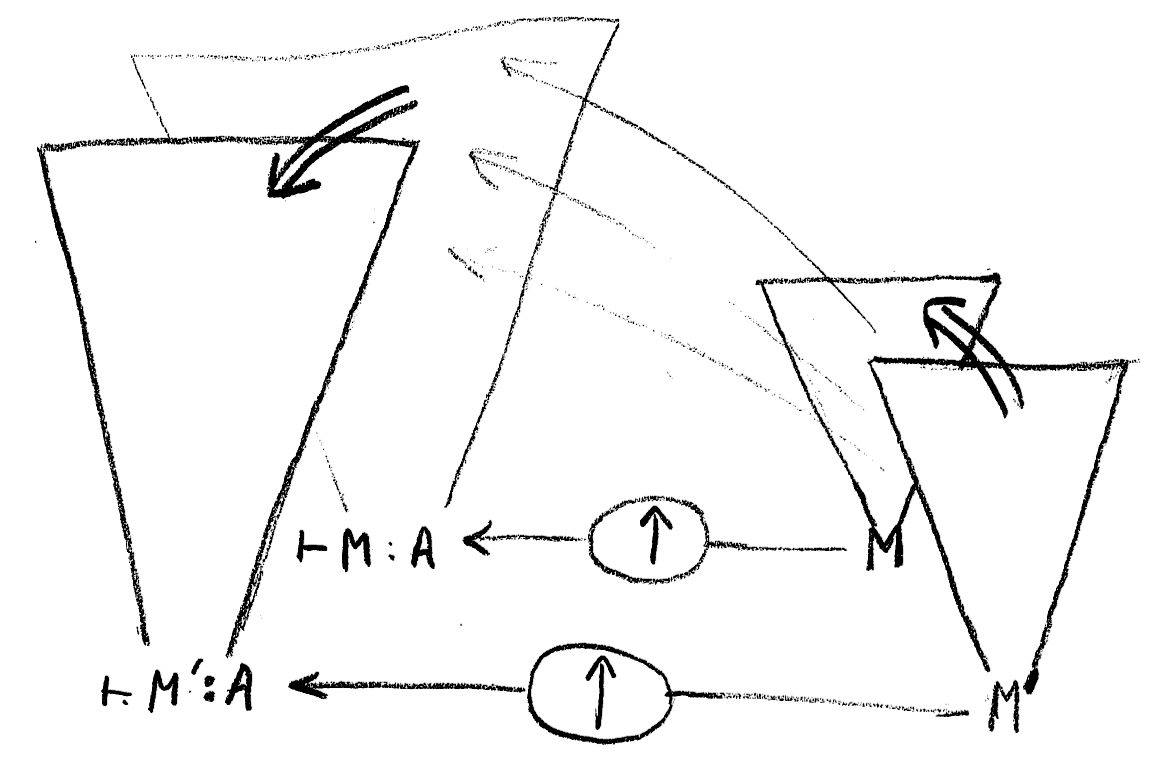
\includegraphics{images/deriv.png}
    \end{center}
  \end{onlyenv}
\end{frame}

\begin{frame}{Back to Problem 1}
  
  \begin{onlyenv}<1>
    \begin{block}{Problem}
      \emph{How to take advantage of the knowledge from previous
        type-checks?}
      \begin{itemize}
      \item Reuse pieces of a computed derivation $\md$
      \item Check only the changed part (the \emph{delta}) of a
        program $M$
      \end{itemize}

      \centering
      \begin{tikzpicture}[node distance=2em, >=latex, hv
        path/.style={to path={-| (\tikztotarget)}}, vh path/.style={to
          path={|- (\tikztotarget)}} ]
        \node[state, tribox] (tc) {$\finfer{}$}; \node (term)
        [left=1cm of tc.north west] {$\delta_{M\to M'}$}; \node (repo)
        [left=1cm of tc.south west] {$\md_M$}; \node (repo2) [right=of
        tc] {$\md_{M'}$};

        \path[->] (term) edge (tc.north west) (repo) edge (tc.south
        west) (tc) edge (repo2) ;
      \end{tikzpicture}
    \end{block}

    \begin{block}{Requirements}
      \begin{itemize}
      \item $\infer{\md_{M'}}{\vdash M' : A}$\quad iff\quad
        $\finfer{(\md_M, \delta_{M\to M'})} = \md_{M'}$
      \item $\finfer{(\md_M, \delta_{M\to M'})}$ computes $\md_{M'}$
        in less than $O(|M'|)$ \small\qquad\flushright (ideally
        $O(|\delta_{M\to M'}|)$)
      \end{itemize}
    \end{block}
  \end{onlyenv}

  \begin{onlyenv}<2>
    \begin{block}{Bidirectional incremental updates}
      % view the derivation as the document we're editing
      % through a view (the program)
      % --> bijective
      \begin{figure}
        \centering
        \begin{tikzpicture}[node distance=4em, auto, >=latex]
          \node (D) {$\mathcal D$}; \node (checkout) [right=of D,
          state, tribox] {$\funname{get}$}; \node (M) [right=of
          checkout] {$M$}; \node (M') [below=3em of M] {$M'$}; \node
          (commit) [state, tribox, left=of M', shape border
          rotate=180] {$\funname{put}$}; \node (D') [below=3em of D]
          {$\mathcal D'$};

          \path[->] (D) edge (checkout) (checkout) edge (M) (M) edge
          [color=red, double] node [name=delta] {$\delta$} (M')
          (commit) edge (D') ;

          \draw[->] (D) |- ++(1,-1) -| (commit) ;

          \draw[->] [out=0, in=0, color=red] (delta) edge (commit);

      \begin{pgfonlayer}{background}
        \node [fill=yellow!30,fit=(D) (D'), label=above:Derivations,
        ellipse] {}; \node [fill=yellow!30,fit=(M) (M'),
        label=above:Programs, ellipse] {}; \node
        [fill=yellow!30,fit=(checkout) (commit), label=above:Lens,
        ellipse, inner sep=0] {};
      \end{pgfonlayer}

    \end{tikzpicture}
  \end{figure}
  \begin{itemize}
  \item $\function{get}{\mathcal D}$ projects derivation $\mathcal D$
    to a program $M$
  \item $\function{put}{\mathcal D, \delta}$ checks $\delta$ against
    $\mathcal D$ and returns $\mathcal D'$
    \begin{itemize}
    \item the incremental type-checker
    \item change-based approach
    \item justification for each change ($\mathcal D'$)
    \end{itemize}
  \end{itemize}
\end{block}
\end{onlyenv}

\end{frame}

\begin{frame}[fragile]{\textcolor{greenish}{Examples}}
    \begin{center}
      \begin{tabular}{r|l}
      \textcolor{greenish}{initial term} &
      {\large\textbf{let} \textit{f x} = \textit{x} + 1
        \textbf{in} \textit{f} 3 / 2} \\[2em]\pause
      \textcolor{greenish}{easy interleave} &
      {\large\textbf{let} \textit{f x} = \alert{2 *} (\textit{x} + 1) \textbf{in}
        \textit{f} 3 / 2} \\[2em]\pause
      \textcolor{greenish}{env interleave} &
      {\large\textbf{let} \textit{f x} =
        (\alert{\textbf{let} \textit{y} = true \textbf{in}} \textit{x} + 1) \textbf{in}
        \textit{f} 3 / 2} \\[2em]\pause
      \textcolor{greenish}{type change} &
        {\large\textbf{let} \textit{f x} = \textit{x} \alert{$>$} 1
          \textbf{in} \cfbox{red}{\textit{f} 3 / 2}}
    \end{tabular}
    \end{center}
\end{frame}

\begin{frame}{In this talk...}

  \begin{onlyenv}<1>
    \begin{block}{The message}
      Generating certificates of well-typing allows type checking
      incrementality by sharing pieces of derivations
    \end{block}

  \begin{block}{The difficulty}
    Proofs are \emph{higher-order objects} (binders, substitution
    property)
    \begin{itemize}
    \item What delta language?
    \item What data structure for derivations?
    \item What language to write synthesis algorithm?
    \end{itemize}
  \end{block}
\end{onlyenv}

\begin{onlyenv}<2->
  \begin{block}{The artifact}
    \sysname{Gasp}: a \emph{language-independent} backend to develop
    certifying, incremental type checkers
    \begin{figure}
      \centering
      \begin{tikzpicture}
        \node[draw=yellow!50!black, fill=yellow!30, rounded corners]
        (input) {
          \begin{tabular}{l}
            syntax \\
            typing rules\\
            checker {\small (untrusted)}
          \end{tabular}
        } ;

        \node[draw=yellow!50!black, fill=yellow!30, rounded corners,
        right=of input] (output) {
          \begin{tabular}{l}
            incremental checker \\
            tactic writing language \\
            version control\ldots \\
          \end{tabular}
        } ;

        \path[->] (input) edge [draw=yellow!50!black, thick, decorate,
        decoration=snake] (output) ;
      \end{tikzpicture}
    \end{figure}
  \end{block}
  \begin{block}{The open question}
    What else can we do with it?
  \end{block}
\end{onlyenv}
\end{frame}

%%% Local Variables: 
%%% mode: latex
%%% TeX-master: "slides"
%%% End: 
